
\subsection{Amplificadores con operacionales}

\label{section:modelo_operacional}

En esta sección analizamos distintas configuraciones con amplificadores operacionales, pero teniendo en cuenta ciertos aspectos de los amplificadores operacionales reales, en particular usamos un modelo lineal, y lo analizamos a bajas/medias frecuencias, sin tener en cuenta en principio el ancho de banda, ni cosas como el \textit{slew rate}, que corresponden a efectos que no se pueden modelar linealmente. El modelo utilizado es el mostrado en la figura~\figref{fig:fig_operational_non_ideal}, como se puede ver, solo consideramos, una ganancia de tensión diferencial de valor finito, una resistencia de entrada también finita y una resistencia de salida mayor a $0$.

\begin{figure}[H] %htb
\begin{center}
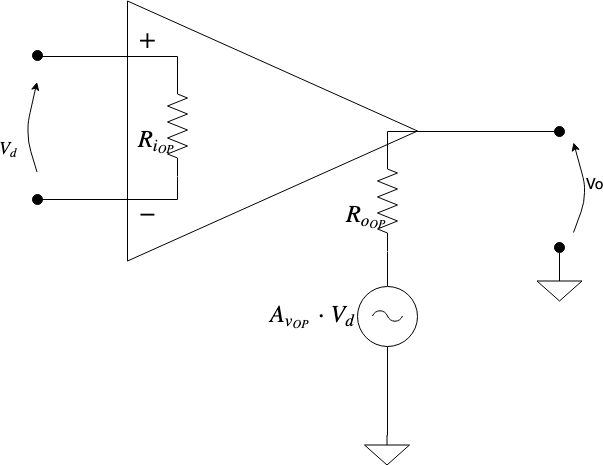
\includegraphics[width=1 \textwidth, angle=0]{./img/operacionales/OP_NONIDEAL_MODEL.png}
\caption{\label{fig:fig_operational_non_ideal}\footnotesize{Modelo lineal de un operacional no ideal.}}
\end{center}
\end{figure}

\vfill

\clearpage

\subsubsection{Amplificador no inversor}

Usando el modelo descripto en la sección~\sectref{section:modelo_operacional} analizamos el circuito mostrado en la figura~\figref{fig:fig_operational_ideal_non_inverter}. El circuito es un amplificador no inversor con amplificador operacional. El análisis que se hará por realimentación, pretende analizar como es la transferencia del mismo con nuestro modelo, y como influye la no idealidad del operacional en la transferencia, para finalmente ver a que se reduce la transferencia al llevar las expresiones al caso ideal.

\begin{figure}[H] %htb
\begin{center}
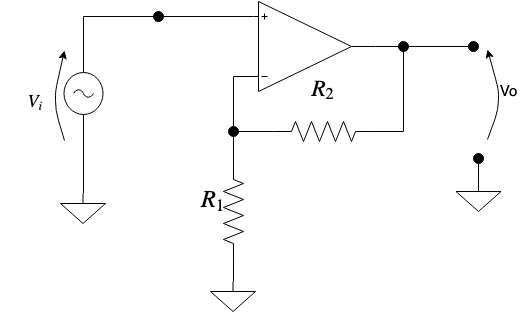
\includegraphics[width=0.5 \textwidth, angle=0]{./img/operacionales/OP_NINV.png}
\caption{\label{fig:fig_operational_ideal_non_inverter}\footnotesize{Amplificador no inversor.}}
\end{center}
\end{figure}


El amplificador es de tensión, para ver esto, se observa que la red de realimentación formada por $R_{1}$ y $R_{2}$, muestrea la tensión a la salida y suma (resta) tensión a la entrada, con lo que se estabiliza la ganancia de tensión. Ya que se trata de realimentación \textbf{serie-paralelo} aplicamos parámetros \textbf{h} al realimentador.



\begin{figure}[H] %htb
\begin{center}
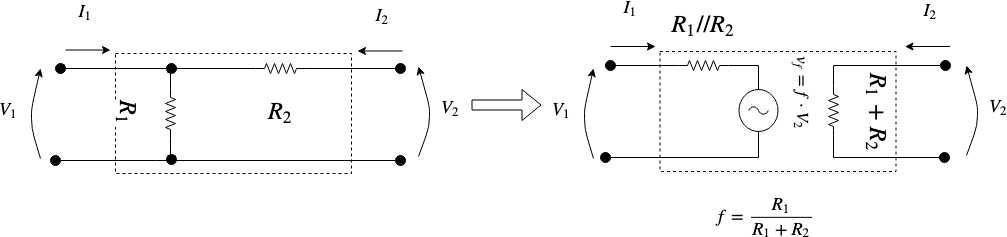
\includegraphics[width=0.9 \textwidth, angle=0]{./img/operacionales/OP_NINV_FEEDBACK.png}
\caption{\label{fig:fig_ninv_feedback}\footnotesize{Aplicando parámetros \textbf{h} al realimentador}}
\end{center}
\end{figure}



Remplazando en el circuito nuestro modelo y el realimentador por el modelo en parámetros \textbf{h}, y reorganizando para llevar el realimentador a su forma ideal, nos queda:


\begin{figure}[H] %htb
\begin{center}
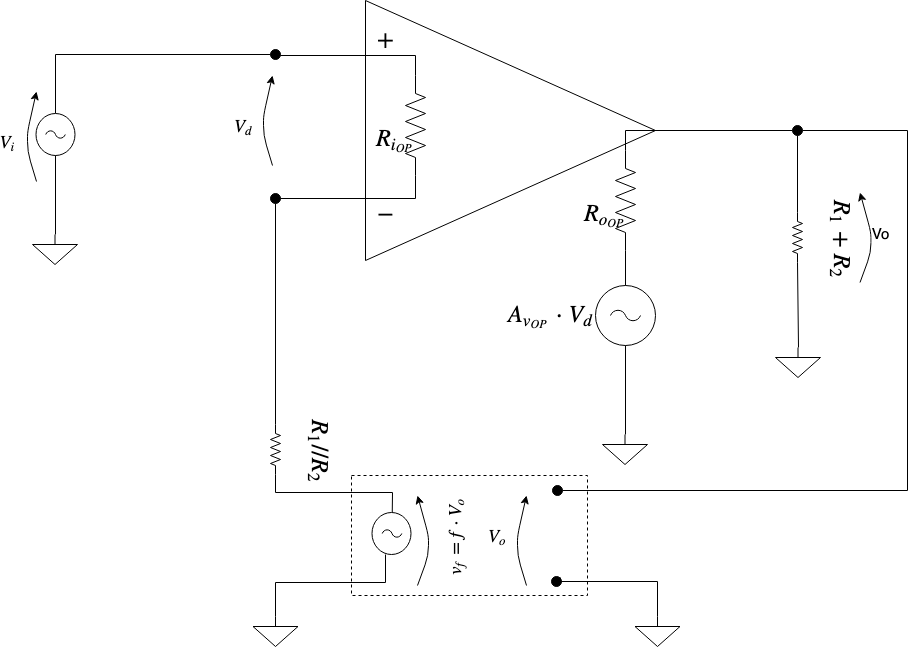
\includegraphics[width=0.9 \textwidth, angle=0]{./img/operacionales/OP_NONIDEAL_MODEL_NINV_FEEDBACK_PARAMETERS.png}
\caption{\label{fig:fig_nideal_ninv_feedback_pars}\footnotesize{Reemplazando en el circuito original junto a nuestro modelo}}
\end{center}
\end{figure}

De este circuito es fácil por inspección obtener la ganancia de tensión a lazo abierto, \quotemarks{a} y las resistencias de entrada y salida a lazo abierto, $R{i_{OL}}$ y $R{o_{OL}}$ respectivamente, se obtiene:


\begin{equation}
a =  \evalat{\frac{V_{o}}{V_{i}}}{f=0} = A_{v_{OP}} \cdot \frac{R_{i_{OP}}}{R_{i_{OP}} + R{1} \parallelresistors R{2} } \cdot \frac{ R_{1} + R_{2}}{R_{o_{OP}} + R_{1} + R_{2} }
\end{equation}

\begin{equation}
f =  \frac{R_{1}}{R_{1} + R_{2}}
\end{equation}

\begin{equation}
R_{i_{OL}} = R_{i_{OP}} + R{1} \parallelresistors R{2}
\end{equation}

\begin{equation}
R_{o_{OL}} = \left( R_{1} + R{2} \right) \parallelresistors R_{o_{OP}}
\end{equation}

Para la ganancia de tensión a lazo cerrado y las resistencias de entrada y salida a lazo cerrado, $R{i}$ y $R{o}$ respectivamente, entonces tenemos:


\begin{equation}
\boxed{ A = \frac{a}{1 + a \cdot f} = \frac{R_{1} + R{2}}{ \left( 1 + \frac{R{1} \parallelresistors R{2}}{R_{i_{OP}}} \right) \cdot \left( \frac{R_{o_{OP}} + R_{1} + R_{2}}{A_{v_{OP}}} + R_{1} \right) } }
\end{equation}


\begin{equation}
\boxed{ R{i} = R_{i_{OL}} \cdot \left( 1 + a \cdot f \right) = \left(  R_{i_{OP}} + R{1} \parallelresistors R{2} \right) \cdot \left[ 1 + \frac{ A_{v_{OP}} \cdot R_{1} \cdot R_{i_{OP}} }{  \left( R_{i_{OP}} + R{1} \parallelresistors R{2} \right) \cdot \left( R_{o_{OP}} + R_{1} + R_{2} \right) } \right] }
\end{equation}


\begin{equation}
\boxed{ R{o} = \frac{R_{o_{OL}}}{1 + a \cdot f} = \frac{\left( R_{1} + R{2} \right) \parallelresistors R_{o_{OP}}}{1 + \frac{ A_{v_{OP}} \cdot R_{1} \cdot R_{i_{OP}} }{  \left( R_{i_{OP}} + R{1} \parallelresistors R{2} \right) \cdot \left( R_{o_{OP}} + R_{1} + R_{2} \right) }} }
\end{equation}


Se obtiene para el caso ideal, cuando $A_{v_{OP}} \longrightarrow \infty$, $R_{i_{OP}} \longrightarrow \infty$ y $R_{o_{OP}} \longrightarrow 0$:

\begin{equation}
\lim_{\substack{A_{v_{OP}} \to \infty \\ R_{i_{OP}} \to \infty \\ R_{o_{OP}} \to 0}} A = 1 + \frac{R_{2}}{R_{1}} 
\end{equation}


\begin{equation}
\lim_{\substack{A_{v_{OP}} \to \infty \\ R_{i_{OP}} \to \infty \\ R_{o_{OP}} \to 0}} R{i} = \infty
\end{equation}


\begin{equation}
\lim_{\substack{A_{v_{OP}} \to \infty \\ R_{i_{OP}} \to \infty \\ R_{o_{OP}} \to 0}} R{o} = 0
\end{equation}


\label{validity_opamp_approx}
Queda ver en cada caso cuando estas aproximaciones son válidas, por ejemplo para el caso del \textit{TL082}, (valores tomados de su hoja de datos~\sectref{datasheet_TL082}), se tiene:

\begin{equation}
\min A_{v_{OP}} \approx 25000
\end{equation}


\begin{equation}
\min R_{i_{OP}} \approx 1 \si[per-mode=symbol]{\tera\ohm}
\end{equation}


\begin{equation}
\max R_{o_{OP}} \approx 100 \si[per-mode=symbol]{\ohm}
\end{equation}

Se puede ver de las expresiones halladas antes, que la ganancia a lazo abierto, \quotemarks{$a$}, será aproximadamente la ganancia de tensión del amplificador operacional, así que en general para valores de resistencias de realimentación en el orden algunos $\si[per-mode=symbol]{\kilo\ohm}$ y valores de realimentación no muy grandes, estas aproximaciones serán muy buenas.

\clearpage

\subsubsection{Amplificador inversor}

En forma similar a la sección anterior, usando el modelo descripto en la sección~\sectref{section:modelo_operacional} analizamos el circuito mostrado en la figura~\figref{fig:fig_operational_ideal_inverter_tr}. El circuito es un amplificador no inversor con amplificador operacional. El análisis que se hará por realimentación, pretende analizar como es la transferencia del mismo con nuestro modelo, y como influye la no idealidad del operacional en la transferencia, para finalmente ver a que se reduce la transferencia al llevar las expresiones al caso ideal.


\begin{figure}[H] %htb
\begin{center}
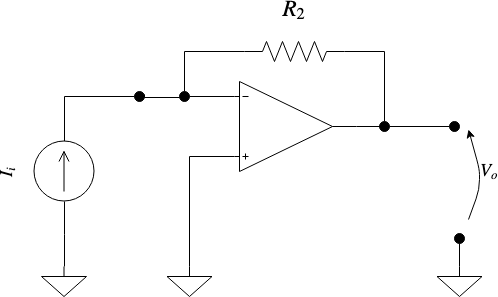
\includegraphics[width=0.5 \textwidth, angle=0]{./img/operacionales/OP_INV_TR.png}
\caption{\label{fig:fig_operational_ideal_inverter_tr}\footnotesize{Amplificador no inversor.}}
\end{center}
\end{figure}

El amplificador es de trans-resistencia, para ver esto, se observa que la red de realimentación formada por $R_{2}$, muestrea la tensión a la salida y suma (resta, ya que la salida invierte respecto de la entrada restadora) corriente a la entrada, con lo que se estabiliza la ganancia de trans-resistencia. Ya que se trata de realimentación \textbf{paralelo-paralelo} aplicamos parámetros \textbf{Y} al realimentador.


\begin{figure}[H] %htb
\begin{center}
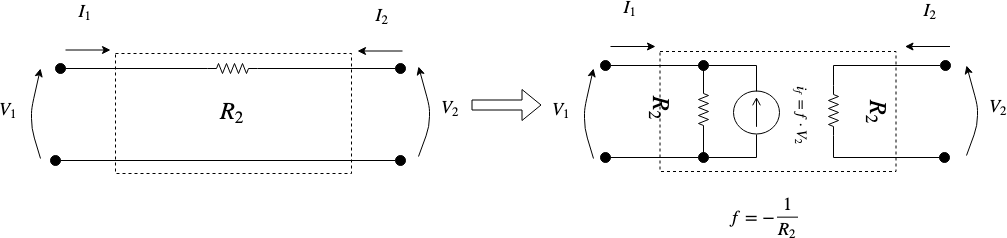
\includegraphics[width=0.9 \textwidth, angle=0]{./img/operacionales/OP_INV_FEEDBACK.png}
\caption{\label{fig:fig_operational_ideal_inverter_tr_feedback}\footnotesize{Aplicando parámetros \textbf{h} al realimentador}}
\end{center}
\end{figure}



Remplazando en el circuito nuestro modelo y el realimentador por el modelo en parámetros \textbf{Y}, y reorganizando para llevar el realimentador a su forma ideal, nos queda:


\begin{figure}[H] %htb
\begin{center}
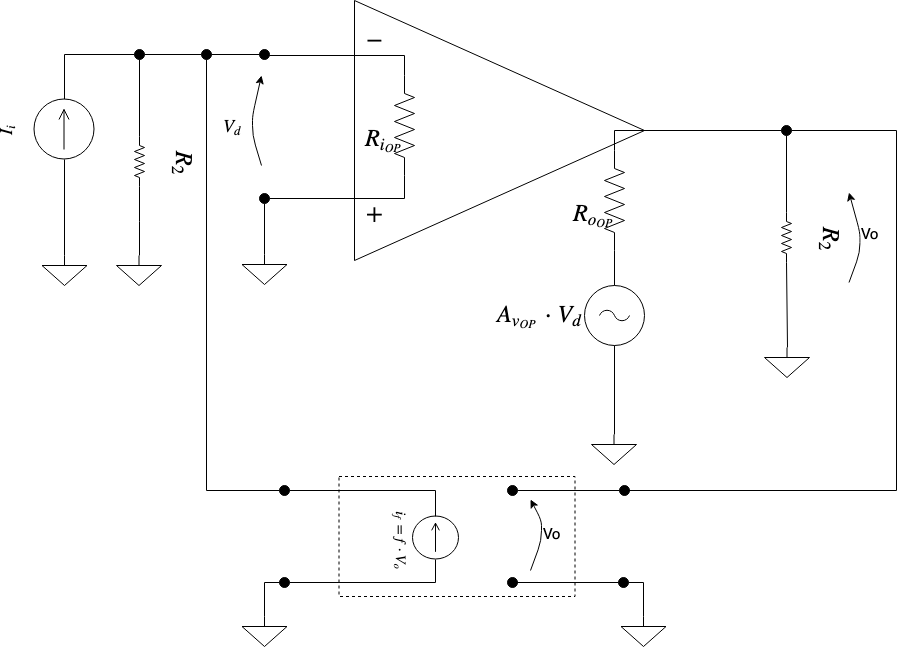
\includegraphics[width=0.9 \textwidth, angle=0]{./img/operacionales/OP_NONIDEAL_MODEL_INV_FEEDBACK_PARAMETERS.png}
\caption{\label{fig:fig_nideal_inv_feedback_pars}\footnotesize{Reemplazando en el circuito original junto a nuestro modelo}}
\end{center}
\end{figure}

De este circuito es fácil por inspección obtener la ganancia de trans-resistencia a lazo abierto, \quotemarks{a} y las resistencias de entrada y salida a lazo abierto, $R{i_{OL}}$ y $R{o_{OL}}$ respectivamente, se obtiene:


\begin{equation}
a =  \evalat{\frac{V_{o}}{I_{i}}}{f=0} = -A_{v_{OP}} \cdot \frac{ R_{2} \cdot R_{i_{OP}} }{ R_{2} + R_{i_{OP}} } \cdot \frac{ R_{2}  }{ R_{2} + R_{o_{OP}} }
\end{equation}

\begin{equation}
f =  -\frac{1}{R_{2}}
\end{equation}

\begin{equation}
R_{i_{OL}} = R_{2} \parallelresistors R_{i_{OP}}
\end{equation}

\begin{equation}
R_{o_{OL}} = R_{2} \parallelresistors R_{o_{OP}}
\end{equation}

Para la ganancia de tensión a lazo cerrado y las resistencias de entrada y salida a lazo cerrado, $R{i}$ y $R{o}$ respectivamente, entonces tenemos:


\begin{equation}
\boxed{   A = \frac{a}{1 + a \cdot f} =  -\frac{ R_{2} }{ 1 + \frac{ \left( 1 + \frac{R_{o_{OP}}}{R_{2}} \right) \cdot \left( 1 + \frac{R_{2}}{R_{i_{OP}}} \right)  }{ A_{v_{OP}}  }  }    }
\end{equation}

\begin{equation}
\boxed{ R{i} = \frac{R_{i_{OL}}}{1 + a \cdot f} =  \frac{ R_{2} \parallelresistors R_{i_{OP}}  }{ 1 + A_{v_{OP}} \cdot \frac{R_{2}}{R_{o_{OP}} + R_{2}} \cdot \frac{R_{i_{OP}}}{R_{i_{OP}} + R_{2}}  }   }
\end{equation}


\begin{equation}
\boxed{ R{o} = \frac{R_{o_{OL}}}{1 + a \cdot f} = \frac{ R_{2} \parallelresistors R_{o_{OP}}  }{ 1 + A_{v_{OP}} \cdot \frac{R_{2}}{R_{o_{OP}} + R_{2}} \cdot \frac{R_{i_{OP}}}{R_{i_{OP}} + R_{2}}  }  }
\end{equation}


Se obtiene para el caso ideal, cuando $A_{v_{OP}} \longrightarrow \infty$, $R_{i_{OP}} \longrightarrow \infty$ y $R_{o_{OP}} \longrightarrow 0$:

\begin{equation}
\lim_{\substack{A_{v_{OP}} \to \infty \\ R_{i_{OP}} \to \infty \\ R_{o_{OP}} \to 0}} A = -R_{2} 
\end{equation}


\begin{equation}
\lim_{\substack{A_{v_{OP}} \to \infty \\ R_{i_{OP}} \to \infty \\ R_{o_{OP}} \to 0}} R{i} = 0
\end{equation}


\begin{equation}
\lim_{\substack{A_{v_{OP}} \to \infty \\ R_{i_{OP}} \to \infty \\ R_{o_{OP}} \to 0}} R{o} = 0
\end{equation}


Para la validez de estas aproximaciones, ver el análisis de la sección~\sectref{validity_opamp_approx}.\\\\

Para este circuito amplificador queda ver el caso en que es usado como amplificador de tensión, como se muestra en la figura~\figref{fig:fig_operational_ideal_inverter}

\begin{figure}[H] %htb
\begin{center}
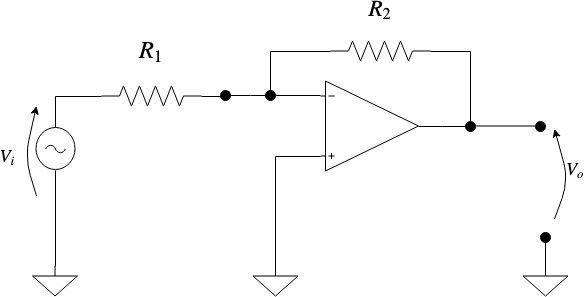
\includegraphics[width=0.5 \textwidth, angle=0]{./img/operacionales/OP_INV.png}
\caption{\label{fig:fig_operational_ideal_inverter}\footnotesize{Amplificador no inversor de tensión.}}
\end{center}
\end{figure}

Usando los resultados anteriores y un simple análisis por inspección se obtiene:

\begin{equation}
\boxed{   A = - \frac{1}{R_{1} + R_{i_{OP}}}    \cdot \frac{ R_{2} }{ 1 + \frac{ \left( 1 + \frac{R_{o_{OP}}}{R_{2}} \right) \cdot \left( 1 + \frac{R_{2}}{R_{i_{OP}}} \right)  }{ A_{v_{OP}}  }  }    }
\end{equation}

\begin{equation}
\boxed{ R{i} = R_{1} + R_{i_{TR}} =  R_{1} + \frac{ R_{2} \parallelresistors R_{i_{OP}}  }{ 1 + A_{v_{OP}} \cdot \frac{R_{2}}{R_{o_{OP}} + R_{2}} \cdot \frac{R_{i_{OP}}}{R_{i_{OP}} + R_{2}}  }   } 
\end{equation}


\begin{equation}
\boxed{ R{o} = \frac{ R_{2} \parallelresistors R_{o_{OP}}  }{ 1 + A_{v_{OP}} \cdot \frac{R_{2}}{R_{o_{OP}} + R_{2}} \cdot \frac{R_{i_{OP}}}{R_{i_{OP}} + R_{2}}  }  }
\end{equation}

La resistencia de salida no se verá afectada respecto al cálculo anterior, y a la entrada tenemos $R_{1}$ en serie con $R_{i_{TR}}$, que es la resistencia de entrada obtenida antes para el amplificador de trans-resistencia. En cuanto a la ganancia de tensión, es solo observar el valor de la corriente que toma el amplificador, que es $\frac{V_{i}}{R_{1} + R_{i_{OP}}}$.\\\\

Se obtiene para el caso ideal, cuando $A_{v_{OP}} \longrightarrow \infty$, $R_{i_{OP}} \longrightarrow \infty$ y $R_{o_{OP}} \longrightarrow 0$:

\begin{equation}
\lim_{\substack{A_{v_{OP}} \to \infty \\ R_{i_{OP}} \to \infty \\ R_{o_{OP}} \to 0}} A = - \frac{R_{2}}{R_{1}} 
\end{equation}


\begin{equation}
\lim_{\substack{A_{v_{OP}} \to \infty \\ R_{i_{OP}} \to \infty \\ R_{o_{OP}} \to 0}} R{i} = R_{1}
\end{equation}


\begin{equation}
\lim_{\substack{A_{v_{OP}} \to \infty \\ R_{i_{OP}} \to \infty \\ R_{o_{OP}} \to 0}} R{o} = 0
\end{equation}


Para la validez de estas aproximaciones, ver el análisis de la sección~\sectref{validity_opamp_approx}.

\clearpage


\subsubsection{Amplificador diferencial}

Analizamos el circuito mostrado en la figura~\figref{fig:fig_operational_ideal_differential}. El circuito es un amplificador diferencial con amplificador operacional. Para ver que se trata de un amplificador diferencial, basta con aplicar superposición, si solo se analiza la salida obtenida para $V_{i_{1}}$, tenemos un amplificador no inversor, si ahora se analiza la salida obtenida para $V_{i_{2}}$, tenemos un amplificador inversor. Dado que el análisis ya se realizó para cada uno de estos amplificadores, usamos estos resultados para obtener la expresión de la ganancia total del amplificador con ambas entradas aplicadas, será necesario aplicar el equivalente de Thévenin a las entradas para reducir el circuito a la forma analizada, también es necesario agrupar los resistores.

\begin{figure}[H] %htb
\begin{center}
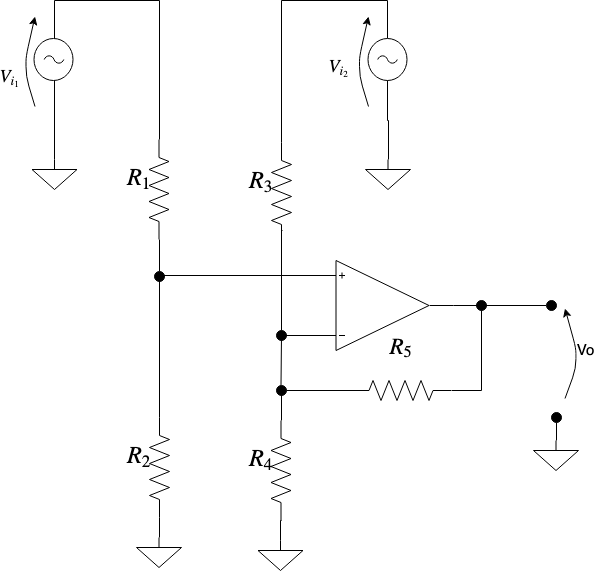
\includegraphics[width=0.5 \textwidth, angle=0]{./img/operacionales/OP_DIFF.png}
\caption{\label{fig:fig_operational_ideal_differential}\footnotesize{Amplificador diferencial.}}
\end{center}
\end{figure}

Si utilizamos las expresiones para el caso ideal de ambos tipos de amplificadores analizados y se obtiene la siguiente expresión luego de reducir:


\begin{equation}
V_{o} = \frac{ R_{2} }{ R_{1}  + R_{2}  } \cdot \left( 1 + \frac{R_{5}}{R_{3}} + \frac{R_{5}}{R_{4}}   \right)  \cdot V{i_{1}} - \frac{R_{5}}{R_{3}} \cdot V{i_{2}}
\end{equation}

Para que la ganancia realmente sea diferencial (proporcional a la diferencia de las entradas) se requiere la siguiente relación entre los valores de los resistores del circuito:


\begin{equation}
\frac{ R_{2} }{ R_{1}  + R_{2}  } \cdot \left( 1 + \frac{R_{5}}{R_{3}} + \frac{R_{5}}{R_{4}}   \right) = \frac{R_{5}}{R_{3}}
\end{equation}

Si se cumple esta relación se tiene:


\begin{equation}
\boxed{A = \frac{V_{o}}{V_{1} - V_{2}} = \frac{R_{5}}{R_{3}}}
\end{equation}

Para la resistencias de entrada (diferencial), por tratarse del caso ideal se tendrá la suma de las resistencias de entradas ideales de ambos amplificadores, y la de salida será igual que para cualquiera de los casos, inversor o no inversor, se tiene entonces:


\begin{equation}
\boxed{R_{i_{d}} = R_{1} + R_{2} + R_{3}}
\end{equation}


\begin{equation}
\boxed{R{o} = 0}
\end{equation}

Igual que antes, para la validez de estas aproximaciones, ver el análisis de la sección~\sectref{validity_opamp_approx}.


\subsubsection{Offset en amplificadores diferenciales con operacionales}

En el caso de un diferencial armado con operacionales, además del offset de tensión que el operacional tenga por su circuito interno, que puede, o no, ser bajo, o compensable, o no, externamente, hay que tener en cuenta el causado por la caída en la resistencia que se ve desde los terminales inversor y no inversor del amplificador operacional. Esta caída es debida a la corriente que toma la entrada del operacional, que a pesar de ser chica, no es nula, incluso en los que tienen entradas con transistores \textbf{FET}. La mejor forma de compensar este offset es asegurarse que ambas entradas vean el mismo valor de resistencia, cuando se considera salida diferencial nula, en ese caso las redes de realimentación conectadas a la salida quedan conectadas a masa del lado de la salida, en esta condición se puede determinar la resistencia total vista por ambas entradas. Al diseñar el circuito se debe tener el cuidado de compensar estos valores.


\subsubsection{Ancho de banda en amplificadores con operacionales}

Los operacionales reales proveen en sus hojas de datos el parámetro \textbf{GP}, que es el producto de la ganancia  por el ancho de banda, \quotemarks{ $A \cdot BW$ }, que se obtiene a lazo cerrado, esta expresión es valida dado que la mayor parte de los operacionales son internamente compensados para comportarse como un sistema de un solo polo. Para el calcular el ancho de banda que se obtiene se debe hacer el siguiente cálculo:

\begin{equation}
\boxed{BW = \frac{GP}{A}}
\end{equation}



